\subsection{FeSe diatomic molecule (NE-AIDMD)}

Transition metal systems are an especially difficult case for most electronic structure methods, and therefore, are an 
important test case for AIDMD. Futhermore, diffusion Monte Carlo is particularly useful in transition-metal systems, where is has been shown to improve the description of energy gaps for the types of orbital excitations used to sample the Hilbert space~\cite{lucas}.
As a test of AIDMD for transition metal systems, we consider an FeSe diatomic molecule with atomic separation 2.43 \AA~in the $z$-direction.
To our knowledge, this FeSe diatom does not exist in nature, but nevertheless serves as a simple illustration of a model for the interaction between a transition metal and ligand.
The bond distance is chosen to match the unconventional superconductor, FeSe~\cite{fese}, and therefore offer insight into a model description for that system in future calculations.

Using the process outlined in Sec.~\ref{sec:theory}, we consider a multiband Hubbard model including one iron $s$, five iron $d$ states, and three selenium $p$ states:
\begin{align*}
  H 
  &=
  \epsilon_{d_{xy}} \sum_{\eta} (n^{d_{xy}}_{\eta}  + n^{d_{x^2-y^2}}_{\eta})
  +
  \epsilon_{d_{z^2}} \sum_{\eta} n^{d_{z^2}}_{\eta} 
  +
  \epsilon_s \sum_{\eta} n^{s}_{\eta} 
  +
  \epsilon_{p_{z}} \sum_{i,\eta} n^{p_{z}}_{i,\eta} 
  \\
  &+ 
  t_{\sigma,d} \sum_{\eta} \left( d_{z^2,\eta}^{\dagger} p_{z,\eta} + \text{h.c.} \right)
  +
  t_{\sigma,s} \sum_{\eta} \left(s_{\eta}^{\dagger}  p_{z,\eta} + \text{h.c.} \right)
  \\
  &+ 
  t_{\pi} \sum_{\eta} \left( d_{xy,\eta}^{\dagger} p_{x,\eta} + d_{yz,\eta}^{\dagger}  p_{y,\eta} + \text{h.c.} \right)
  \\
  &+
  U_d \sum_{i} n^{d}_{i,\uparrow} n^{d}_{i,\downarrow} 
  +
  J_d \sum_{i\ne j} S_i \cdot S_j.
  +
  E_0
\end{align*}
Here, $\eta$ represents the spin index and $i$ represents orbital index.
The $\epsilon_i$ terms represent single-particle orbital energies, while the $U_d$ is an on-site interaction among the $d$ orbitals and the $J_d$ is a Hund's coupling among the $d$ orbitals.
$E_0$ is an overall energy shift compared to the \textit{ab initio} hamiltonian.
This set of parameters was chosen based on the matching pursuit method described in Sec.~\ref{sec:theory}.

The parameters resulting from NE-AIDMD are presented in Table~\ref{tab:fese}. 
To illustrate the effect of using DMC to sample the wave functions, we also compare the results to the corresponding results from using the DFT calculations used to generate the trial wave functions. 
The states sampled consisted of singles and doubles excitations from PBE calculations with total spin 0, 2, and 4, which were then relaxed via a DMC projection.
The standard deviation of energy of the states sampled was 1.11 eV.
The $J$, $U_d$, and $t_\sigma$ were selected first by matching pursuit, as they correlated the most with the energy of the states.
A model with just these three parameters was able to achieve a root mean square error (RMSE) of 0.77 eV.
The other parameters were necessary to describe a subset of low-energy states that generally involved excitations from iron $3d$ states to iron $4s$ states. 
After adding these additional parameters, the RMSE reduced to 0.60 eV.

\BDB{Can possibly add DFT results for comparison/importance of accurate corrleation}.

The results of the parameter fit are consistent with intuition for this model. 
The $J$, $U_d$, and $t_\sigma$ are selected by matching pursuit first, and have the lowest uncertainties.
Correspondingly, the magnetic state of the iron, the interaction between $d$ electrons on the iron, and the bonding with the selenium are the most important differences between the states.
The sign of $J$ is consistent with Hund's coupling. 
The signs of $t_\sigma$ is positive, consistent with Se located in positive $z$ with respect to Fe. 
Likewise $t_\pi$ is negative corresponding to positive overlap integrals, and is smaller than $t_\sigma$ in magnitude.
The signs of each $\epsilon_i$ are describing differences in energy from exciting $d$ electrons in the iron to the 4s state.
A comparison of the model and \textit{ab initio} energies is shown in Fig. \ref{fig:fese}.
The fit is quite good considering the localized models will suffer from orbitals relaxations effects above. 

\begin{table}[ht]
\label{tab:fese}
\centering
\begin{tabular}{|c|c|}
\hline
  $\epsilon_d$       &  -0.8(2) \\
  $\epsilon_\pi$     &  0.35(8) \\
  $\epsilon_s$       &  2.4(3)  \\
  $\epsilon_\sigma$  &  -0.5(1) \\
  $t_\sigma$         &  2.6(2)  \\
  $t_\pi$            &  -0.7(2) \\
  $U_d$              &  2.9(2)  \\
  $J$                &  -0.44(4) \\
\hline
  RMSE [eV] & 0.60 \\
\hline
\end{tabular}
\caption{Downfolding parameters for FeSe diatomic molecule.}
\end{table} 

\begin{figure*}[htb]
\centering
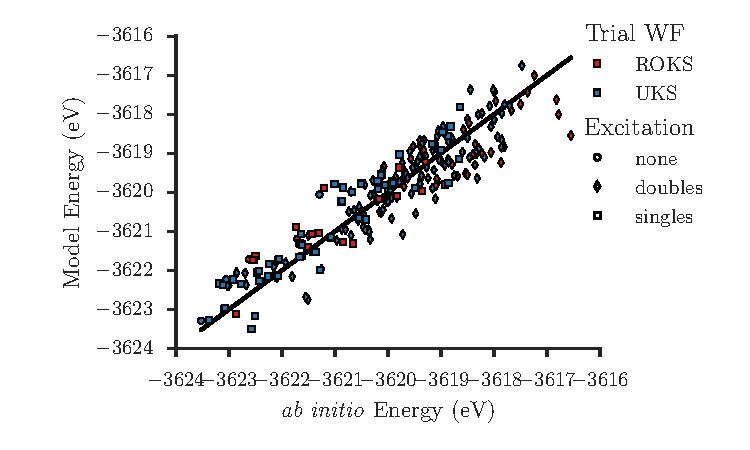
\includegraphics[width=0.7\textwidth]{./Figures/fese.pdf}
  \caption{
    Comparison of \textit{ab initio} (x-axis) and fitted energies (y-axis) of the FeSe diatomic molecule.
    \BDB{Possibly simplify this and/or add DFT results for comparison.}
  }
  \label{fig:fese}
\end{figure*}
